\section{Question 1}

Determine what the following network computes. (To be more precise, determine the output function calculated by the unit at the final time step.) The size of other outputs is not important. All biases are zero. Assume the inputs are integers, and the length of the input sequence is even. Also, consider the activation function to be a sigmoid.

\begin{figure}[H]
    \centering
    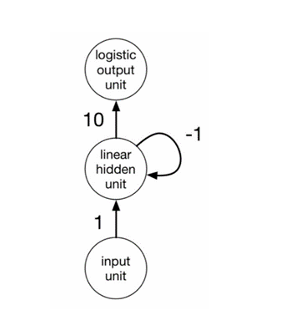
\includegraphics[width = 0.4\textwidth]{Q1.png}
    \caption{Network of Question 1}
\end{figure}
\begin{qsolve}
    \begin{qsolve}[]
Let the input sequence be denoted as \( x_1, x_2, \dots, x_T \), where \( T \) is the length of the input sequence (assumed to be even). The hidden state at time \( t \) is denoted as \( h_t \), and it is updated as follows:

\[
h_t = x_t - h_{t-1}
\]

where \( h_0 = 0 \) (since all biases are zero).

At the final time step \( T \), the hidden state is:

\[
h_T = x_T - h_{T-1}
\]

Substituting recursively, we find:

\[
h_T = x_T - (x_{T-1} - (x_{T-2} - \cdots - (x_2 - x_1)))
\]
\splitqsolve[\splitqsolve]
This simplifies to:

\[
h_T = x_T - x_{T-1} + x_{T-2} - x_{T-3} + \cdots + (-1)^{T+1} x_1
\]

The pattern indicates that \( h_T \) is the alternating sum of the input sequence \( x_1, x_2, \dots, x_T \).

Next, the output of the logistic unit is given by:

\[
y_T = \sigma(10h_T)
\]

Substituting \( h_T \), the output becomes:

\[
y_T = \sigma\left(10 \cdot \sum_{t=1}^T (-1)^{t+1} x_t\right)
\]

where \( \sigma(x) \) is the sigmoid activation function.

Thus, the network computes the alternating sum of the input sequence, scales it by \( 10 \), and applies the sigmoid function.

    \end{qsolve}
\end{qsolve}